\subsection{Considerazioni}
\begin{frame}
    \frametitle{Considerazioni}
    MIFARE Classic non rappresenta una piattaforma sicura per lo sviluppo di applicazioni contactless, e in
    particolare è inadatto ad applicazioni relative a micropagamenti\pause

    Durante la progettazione della tecnologia sono stati commessi gravi errori che, data la banalità di alcuni,
    potrebbero essere stati inseriti con scopi malevoli~\cite{Courtois2009TheDS}
\end{frame}

\subsubsection{RNG}
\begin{frame}
    \frametitle{Miglioramenti - RNG}
    La maggioranza degli attacchi utilizza la predicibilità del RNG. \pause
    
    La soluzione in questo caso è di utilizzare un TRNG disponibile in hardware, a costo di spazio su silicio e di costi pecuniari maggiorati.\pause

    Un miglioramento parziale potrebbe avvenire utilizzando un LFSR da 32 bit e non 16, aumentando così le possibili combinazioni al fine di rallentare gli attacchi.
\end{frame}

\subsubsection{TRNG}
\begin{frame}[allowframebreaks]
    \frametitle{TRNG}
    \begin{figure}
        \centering
        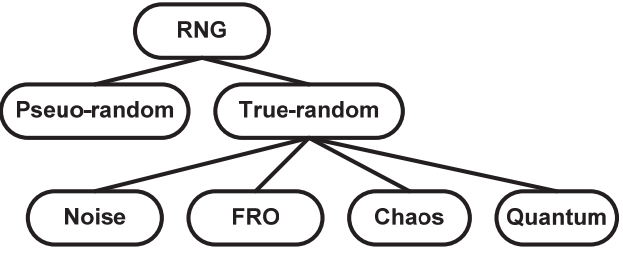
\includegraphics[width=.3\textwidth]{rngFamilies.png}
        \caption{Famiglie di RNG}
    \end{figure}
    È possibile creare TRNG basati sul rumore dell'ambiente in relativamente poco spazio e a basso costo.~\cite{fermevc2016low}

    Il concetto principale nella generazione consiste nel generare un rumore bianco casuale dall'ambiente circostante o da una giunzione PN.

    Ciò permette di generare valori metastabili all'ingresso di flipflop 
    che potranno generare risultati non deterministici per gli effetti elettronici interni.

    \begin{figure}
        \centering
        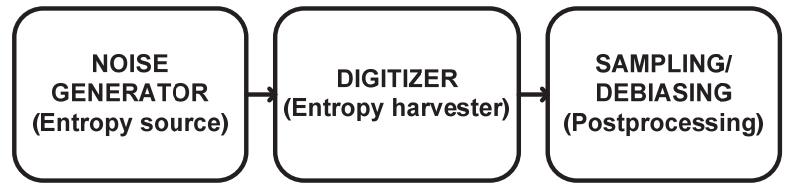
\includegraphics[width=.5\textwidth]{trng_noise.png}
        \caption{Processo di generazione di un numero casuale.}
    \end{figure}

    Da quanto riportato da~\cite{fermevc2016low} è possibile implementare un TRNG con componenti comuni e a bassissimo costo (LM393) e un microcontrollore (già presente nel tag).

    \begin{figure}
        \centering
        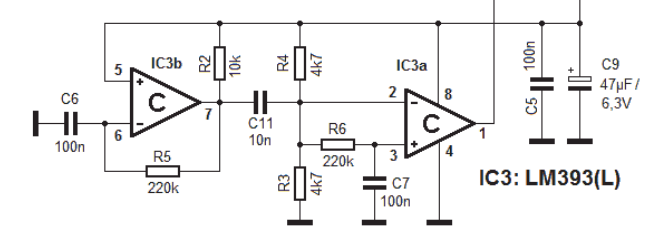
\includegraphics[width=.5\textwidth]{trng_schematic.png}
        \caption{Schema elettronico del generatore di rumore.\cite{fermevc2016low}}
    \end{figure}

    Senza andare nel dettaglio del funzionamento, il primo comparatore viene utilizzato come vera e propria fonte di entropia, mentre il secondo viene utilizzato come digitalizzatore per avere un output binario.

    \begin{figure}
        \centering
        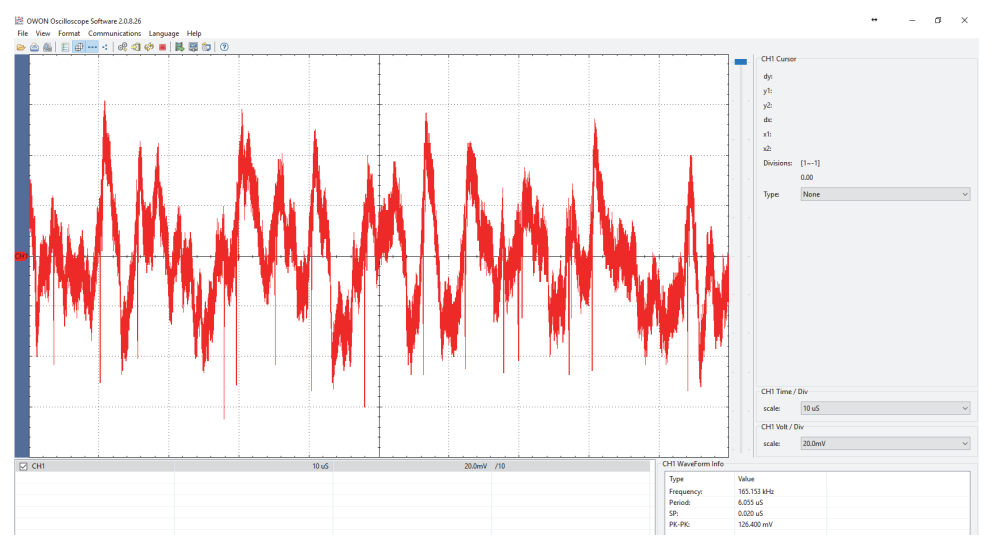
\includegraphics[width=.4\textwidth]{trng_noise_oscope.png}
        \caption{Traccia del rumore generato.\cite{fermevc2016low}}
    \end{figure}

    Svantaggi: Il consumo di un generico TRNG si aggira sui 100mW~\cite{fermevc2016low}. Sono necessarie modifiche e ottimizzazioni per l'inclusione in un tag passivo.
\end{frame}

\subsubsection{LFSR}
\begin{frame}
    \frametitle{Miglioramenti - LFSR}
    Alcune vulnerabilità sono causate dalla funzione di filtraggio del LFSR (Slide~\ref{sec:filter-fn}).
    A tal fine potrebbe essere vantaggiosa un'implementazione dove il cifrario venga sostituito da un modello crittograficamente sicuro.
    
    Una valida proposta potrebbe essere GRAIN-128, cifrario ideato sostanzialmente per ambienti e dispositivi a basso costo e bassissima area occupata\cite{gren2011grain}\cite{sonnerup2019efficient}
\end{frame}

\begin{frame}
    \frametitle{Miglioramenti - LFSR}
    Restano però alcune problematiche:
    \begin{itemize}
        \item <1-> Grain necessita di una chiave di 128bit\newline
                A tal fine è possibile caricare un valore randomico a seguire della chiave nel cifrario per garantire più entropia dei processi di autenticazione.
        \item <2-> Alternativamente sarebbe necessario aumentare la lunghezza della chiave.\newline Per fare ciò sarebbe poi necessario modificare la struttura di memoria oppure ridurre lo spazio consentito ai dati del tag.
    \end{itemize}
\end{frame}
\note{
    In ogni caso la lunghezza della chiave di 48 bit è da considerarsi non siura, tanto quanto la tecnologi hardware.
}

\subsubsection{Grain128}
\begin{frame}[allowframebreaks]
    \frametitle{Grain128a}
    \textbf{Vantaggi}
    \begin{itemize}
        \item <1-> Crittograficamente sicuro
        \item <2-> Può includere un MAC
    \end{itemize}

    Grain utilizza chiavi da 128 bit e IV da 96 bit, mentre la struttura interna è composta da un LFSR da 128 bit e da un NLFSR anch'esso da 128 bit

    \begin{figure}
        \centering
        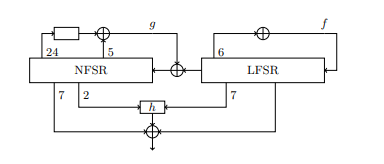
\includegraphics[width=.5\textwidth]{grain128.png}
        \caption{Schema logico di Grain128/Grain128a}
    \end{figure}

    All'interno di Grain è possibile trovare due registri a scorrimento, uno lineare e uno non lineare.

    In aggiunta $h$ è una funzione non lineare che contribuisce all'output.
\end{frame}

\begin{frame}
    \frametitle{Grain128a iii}

    Per inizializzare il cifrario, una chiave da 128bit e un IV da 96 bit vengono inseriti nell'NLFSR e nel LFSR rispettivamente, completando l'LFSR con una costante.
\end{frame}

\begin{frame}
    \frametitle{Grain128a - Autenticazione i}

    Per autenticare il tag è possibile utilizzare il cifrario Grain128a:

    Il keystream è dato da $y_{64+2n}$ ovvero dai bit dispari dell'output scartando i primi 64.

    \begin{figure}
        \centering
        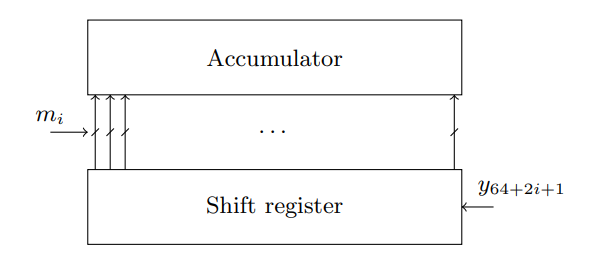
\includegraphics[width=.5\textwidth]{grain128auth.png}
        \caption{Schema logico dell'autenticazione utilizzata da Grain128a}
    \end{figure}
\end{frame}

\begin{frame}
    \frametitle{Grain128a - Autenticazione ii}

    Assumiamo di avere un messaggio $\bar{m} = m_0,m_1,...,m_{L-1}$ di lunghezza $L$.

    Per garantire che $\bar{m}$ e $\bar{m}||0$ abbiano risultato diverso (attacchi di tipo extension) poniamo $m_L = 1$\pause

    \textbf{Inizializzazione}

    Il registro accumulatore viene inizializzato con i primi 32 bit del keystream, il registro a scorrimento viene inizializzato con i successivi 32.\pause

    \textbf{Autenticazione}

    Codificando il messaggio, il registro a scorrimento sarà aggiornato ogni due bit del keystream ($r_{i+31 = y_{64+2i+1}}$) mentre l'accumulatore sarà aggiornato secondo $a_{i+1} = a_i \oplus m \cdot r$
\end{frame}
\note{
    Il risultato dell'autenticazione è quindi il valore finale dell'accumulatore che sarà uguale sia per la cifratura che la decifratura del messaggio.
}

\begin{frame}
    \frametitle{Miglioramenti - ALGORITMO}
    Una soluzione più drastica è rappresentata dal cambio del circuito di cifratura, passando a un'implementazione AES a basso costo.\cite{feldhofer2005aes}

    In questo caso resta la problematica della gestione di chiavi a 128 bit.
\end{frame}

